\newpage
\begin{song}{title={``1788''}, music={Jacek Kaczmarski}}
    \small
    \begin{intro}
        \writechord{F} \writechord{B} \writechord{F} \writechord{C} \\ 
        \writechord{F} \writechord{B} \writechord{F} \writechord{C} \writechord{F}
    \end{intro}
    \begin{multicols}{2}
    \begin{verse}
        ^{F}Ta pierwsza morska ^{B}podróż do Australii! \\
        ^{F}Łotry przy burtach, prosty^{C}tutki w kojach \\
        ^{F}Wszyscy się bali, łk^{B}ali i rzygali \\
        ^{F}W drodze do raju. Przewrot^{C}ności Twoja \\
        ^{d}Panie, coś w jeszcze nam niezn^{g}anych planach \\
        ^{d} Miał czarne diabły strzeg^{a}ące wybrzeży \\
        ^{B}Edenu, który prz^{C}eznaczyłeś ^{F}dla nas \\
        A w kt^{B}óry nikt, prawdę ^{C}mówiąc, nie ^{d}wierzył! \\
        \\
        ^{d} ^{B} ^{F} ^{C}
    \end{verse}
    \begin{verse}
        Czym żeśmy, marni, zasłużyli na to? \\
        Ten, co zawisnąć miał za kradzież płaszcza \\
        Płakał nad swoją niechybną zatratą \\
        Nie widział Ciebie w robaczywych masztach \\
        Statku, co tylko był więzieniem nowym \\
        Tej co kupczyła ciałami swych dziatek \\ 
        Ani przez mgnienie nie przyszło do głowy \\
        Że to nadziei --- nie rozpaczy statek
    \end{verse}
    \begin{verse}
        Niejeden żołnierz z ponurej eskorty \\
        Bo czym się ich los od naszego różnił? \\ 
        Wiedział, że nigdy już nie ujrzy portu \\
        Gdzie go podejmą karczmarze usłużni \\ 
        I płatne dziewki; że zabraknie rumu \\
        Zanim do celu przygnasz okręt szparki \\
        Z marynarzami pili więc na umór \\
        I --- wbrew zakazom --- grali o więźniarki
    \end{verse}
    \vfill\null\columnbreak{}
    \begin{verse}
        Prawda, nie wszyscy próby Twe przetrwali \\
        Ale też ciężkoś nas doświadczał, Panie \\
        Nie oszczędzałeś nam wysokiej fali \\ 
        Za którą mnogim przyszło w oceanie \\
        Zakończyć żywot; innym dziąsła zgniły \\
        Wypadły zęby, rozgorzały wrzody \\ 
        Więc znaczą nasz zielony szlak mogiły \\
        Szkorbutu, szału, francuskiej choroby
    \end{verse}
    \begin{verse}
        Nikt nie odnajdzie w ruchomych otchłaniach \\
        Ciał nieszczęśników --- oprócz Ciebie, Boże \\
        Ich żywot grzeszny epitafiów wzbrania \\
        Lecz --- ukarani. Więc wystarczy może \\ 
        Żeś się posłużył straszliwym przykładem \\
        Oni naprawdę dotarli do piekieł \\
        A umierając nie wierzył z nich żaden \\
        Że w swym cierpieniu umiera --- człowiekiem
    \end{verse}
    \begin{verse}
        Ląd nam się wydał niegościnny, dziki \\
        Łotr bez honoru, kobieta sprzedajna \\
        Z dnia na dzień --- jak się stać ma osadnikiem \\
        Nieznanych światów? Bo rozpoznać Raj nam \\
        Nie było łatwo; znaleźć w sobie siłę \\
        Wbrew przeciwnościom, bez słowa zachęty \\
        By mimo wszystko żyć --- nim nam odkryłeś \\ 
        Kraj szczodry w zboże, złoto i diamenty
    \end{verse}
    \begin{verse}
        ^{d}Łajdacki pomiot, łot^{g}rowskie nasienie \\
        ^{d}Czerpiąc ze spichrza Twoich d^{a}óbr wszelakich \\
        ^{B}Choć tyle wiemy w^{C}łasnym doświadcz^{F}eniem \\
        ^{d}W nas jest Raj, Pi^{B}ekło --- ^{F}i do obu szl^{C}aki \\
        ^{d}W nas jest Raj, Pi^{B}ekło --- ^{F}i do obu szl^{C}aki \\
        ^{d}W nas jest Raj, Pi^{B}ekło --- ^{F}i do obu szl^{C}aki \\
        \\
        \writechord{d} \writechord{B} \writechord{F} \writechord{C}
    \end{verse}
    \end{multicols}
    %\begin{center}
    %    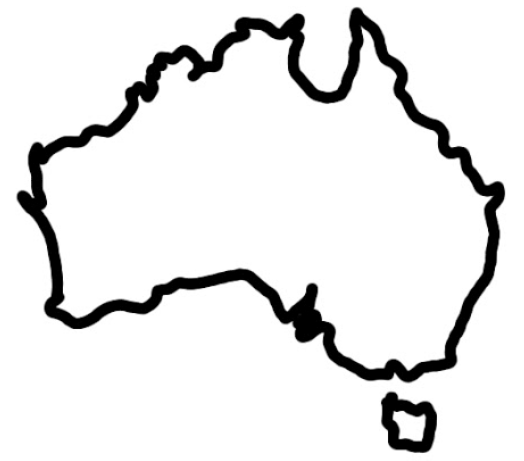
\includegraphics[width=0.15\textwidth]{images/1788.png}  
    %\end{center}
\end{song}
\fancyfoot[LO,RE]{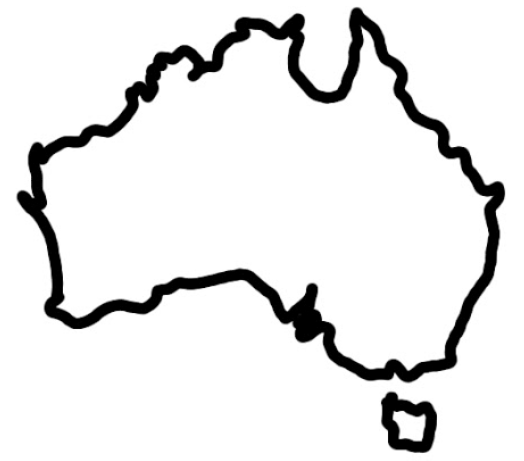
\includegraphics[width=2cm]{images/1788.png}}
